\subsection{Algemeen concept}
De testen maken gebruik van een simpele server waar clients op kunnen verbinden. De client kan vervolgens het absolute tijdverschil meten met een atomische wereldklok.

Eerst en vooral is er een vertraging tussen een aangesloten client en de server, de {\it ping}. Dit is gemeten in milliseconden. De testen meten de vertraging door een bericht met de actuele tijd te verzenden van de server naar de client, en terug. De vertraging is dan de verzonden tijd afgetrokken van de actuele tijd waarmee de ping verkregen is.
In figuur \ref{ping} is de informatieoverdracht zichtbaar. De server berekent de servertijd (TS1) door middel van een API die de exacte wereldtijd teruggeeft, verzonden naar de client en teruggekregen. De uiteindelijke ping is: \[ping = TS2 - TS1\] met TS2 de actuele tijd berekent in de server TS2

\begin{figure}[h]
\centering
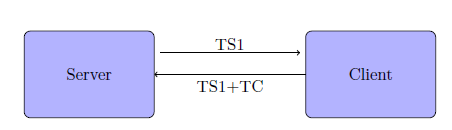
\includegraphics[scale=0.8]{img/img.png}
\caption{Ping} \label{ping}
\end{figure}


Het is niet gegarandeerd dat de klokken van de clients allemaal gesynchroniseerd zijn met de server. Bij het terug verzenden van de client naar de server wordt de clienttijd (TC) bij het bericht gezet.  Met deze TC en de berekende {\it ping} is het mogelijk het tijdsverschil tussen de client en de server te bepalen ($DeltaTime$).
\[DeltaTime = (TC+ping/2) - TS2\]
Het verslag zal deze data bekijken vergelijken tussen verschillende browsers en besturingssystemen.

\subsection{UDP vs TCP}

UDP heeft in tegenstelling tot TCP geen verbinding nodig tussen bijvoorbeeld server en client. TCP zal garanderen dat data correct aankomt door middel van foutopsporing en zal ook in de goede volgorde binnenstromen. Om geen pakketten te verliezen zal TCP deze in een {\it receive buffer} steken en zal de applicatie de ontvangen data pas lezen als ze er klaar voor is. Tegenover UDP waar de data continu zal binnenstromen, ontvangen of niet. Deze zal ook niet aan foutopsporing doen en de juiste volgorde is niet gegarandeerd. Het is duidelijk dat UDP veel sneller is doordat deze minder stappen bevat. Dit is ook de reden dat het NTP protocol UDP zal gebruiken in plaats van TCP. Het is logisch dat voor een simpele synchronisatie tussen client en server geen complex protocol nodig is. Socket.io gebruikt het TCP protocol.

\subsection{Drift en skew}

Drift zal ervoor zorgen dat een clock uit sync valt met een referentie. Windows lost dit op met een wekelijkse resync (het tijdsverschil zal dus op een sawtooth diagram lijken) terwijl Mac OSX rekening zal houden met de clock skew om zo beter in sync te blijven.
Clock skew is het verschil van tijd van een clock signaal tussen 2 componenten (zie figuur \ref{skew1} \cite{skew}).

\begin{figure}[h]
\centering
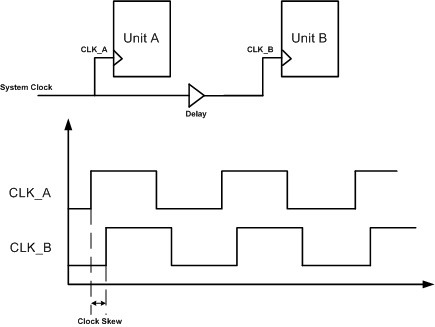
\includegraphics[scale=0.7]{img/skew.jpg}
\caption{Ping} \label{skew1}
\end{figure}


Clock skew kan problemen geven voor correct timings, en zoals eerder vermeld zal OSX dit tegen gaan via software. We zullen niet verder gaan over de problemen van skew en OSX. 


\subsection{Analyse van de data}

Het is duidelijk dat Windows de meeste fluctuaties geeft. 
















